\documentclass{article}
\usepackage[utf8]{inputenc}
\usepackage[spanish]{babel}
\usepackage{listings}
\usepackage{graphicx}
\graphicspath{ {images/} }
\usepackage{cite}
\begin{document}

\begin{titlepage}
    \begin{center}
        \vspace*{1cm}
            
        \Huge
        \textbf{PARCIAL 2}
            
        \vspace{0.5cm}
        \LARGE
        INFORME
            
        \vspace{1.5cm}
            
        \textbf{Michael Stiven Zapata Giraldo\\Brayan Steven Avila Marin}
            
        \vfill
            
        \vspace{0.8cm}
            
        \Large
        Despartamento de Ingeniería Electrónica y Telecomunicaciones\\
        Universidad de Antioquia\\
        Medellín\\
        Septiembre de 2021
            
    \end{center}
\end{titlepage}

\tableofcontents
\newpage
\section{ Clases implementadas }\label{intro}
Creamos una clase llamada ficheros con la cual tenemos unos metodos para manipular las matrices de colores R G B para hacerle el submuestreo y posteriormente llevar el resultado a un archivo TXT el cual tendra la informacion para copiar en el Tinkerkad.

\section{Estructura final de las clases implementadas}  
\begin{itemize}
\item Se define la clase ficheros)
\item Se crean varios metodos para crear y manipular los txt que seran la salida del programa
\item Se crea tambien un metodo para el submuestreo y se escribe en el txt simultaneamente.
\item Se invoca la clase ficheros en el main donde por medio de unos objetos se hace uso de dichos metodos.

\end{itemize}

\section{Estructura del circuito montado}

\begin{itemize}
\item Se amplia la matriz de led a un tamañao de 16x16 para tener una mejor representacion en los leds.
\item Usamos un arduino uno para el montaje el el puerto digital 4
\item Usamos una fuente de poder para suministrar energia a las tiras led RGB
\item Para conectar cada tira se una un cable desde el pin digital  4 del arduino y se conecta a la entrada DIN y luego por la salida DO usamos un cable para conectar la siguiente tira led por el DIN, asi sucesivamente conectamos las tiras para manipularlas por puerto digital de arduino.
\item Establecer una fuente de energia o  fuente de voltaje de 5V/1A.
\item Del arduino llevamos tierra a la fuente de voltaje y de esta misma scamos tierra para la tira led, asi mismo con la potencia desde la fuente hacia la tira led. Ahora conectamos en pueste los 5v de cada tira y la tierra de cada tira para que queden correctamente alimentados.
\item Utilizaremos la clase setPixelColor para apagar algunos leds y la clase show para actuaizar los leds.

\end{itemize}

\section{Problemas presentados durante la implementacion}

\begin{itemize}
\item Problemas con las ramas de Github.
\item La necesidad de usar memoria dinamica para las matrices de color, se investigo para dar solucion y poder implementar memoria dinamica en matrices bidimensionales.
\item Problemas para ubicar los pixeles necesarios para reducir la imagen.
\item Se tuvo que cambiar el tamaño de la matriz de leds para tener una mejor visualizacion.


\end{itemize}
\section{ Manual de uso}
\begin{itemize}
    \item Ejecute la aplicacion
    \item El programa le pedira el nombre de la imagen debe escribirla con la extension .jpg
    \item El programa se encargara de cargar la imagen y procesarla en un archivo .txt
    \item Cuando finalice la ejecucion del programa abra el archivo .txt
    \item Copie el contenido de este archivo y llevelo a el proyecto de tinkerkar y copielo antes del void setup
    \item inicie la simulacion del tinkerkad.
\end{itemize}


\section{Módulos de código implementado donde se evidencie la interacción entre las
diferentes clases} 

\begin{figure}[ht]
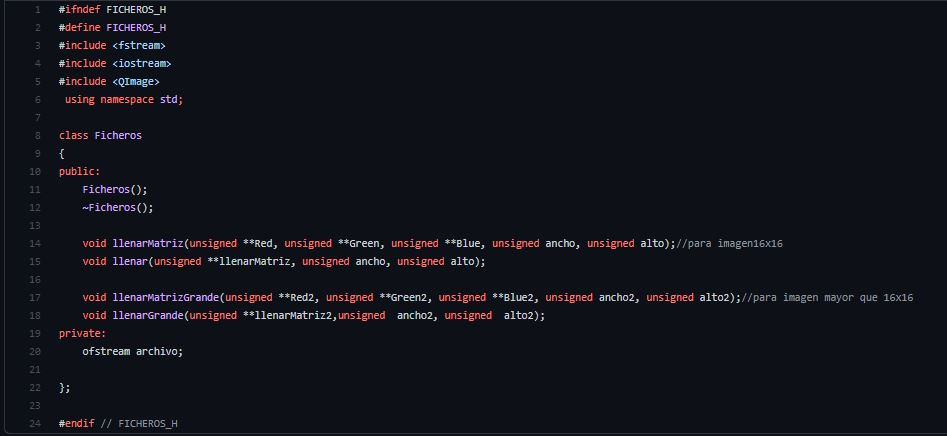
\includegraphics[width=11cm]{Imagenes/Clase ficheros.png}
\centering
\caption{Clase ficheros}
\label{fig:Clase ficheros}
\end{figure}

\begin{figure}[ht]
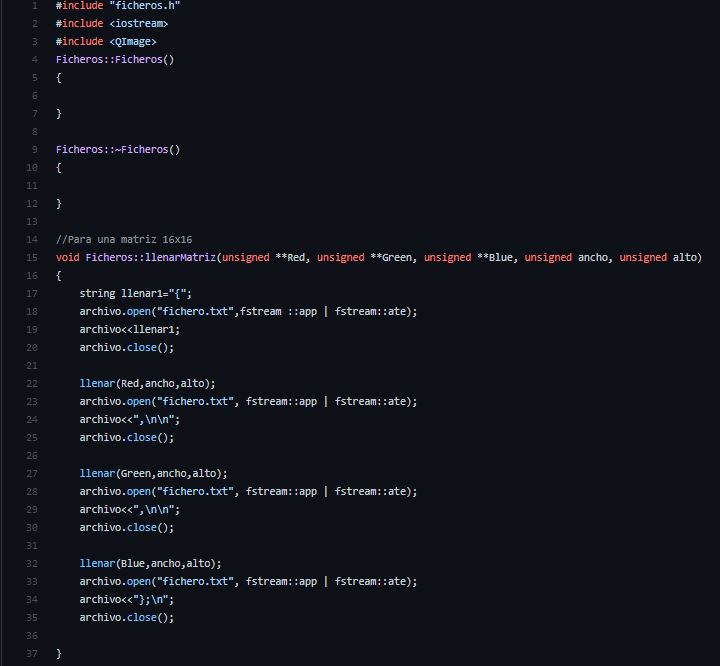
\includegraphics[width=10cm]{Imagenes/Metodos de la clase ficheros.png}
\centering
\caption{Metodos de la clase ficheros}
\label{fig:Metodos de la clase fichero }
\end{figure}

\begin{figure}[ht]
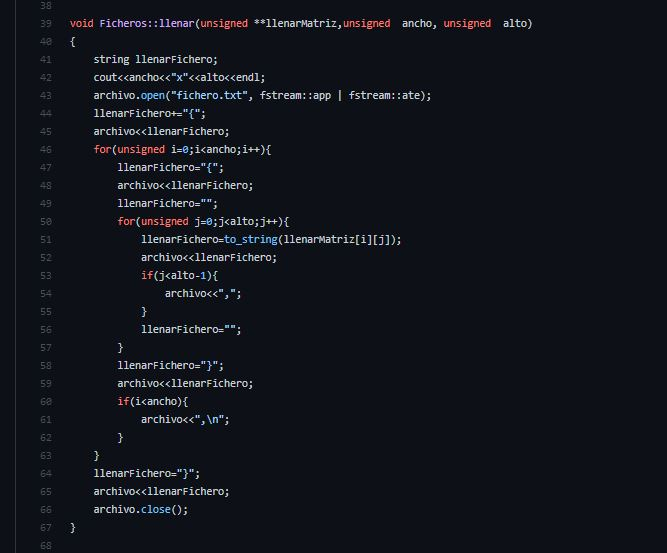
\includegraphics[width=10cm]{Imagenes/Metodos de la clase ficheros2.png}
\centering
\caption{Metodos de la clase ficheros}
\label{fig:Metodos de la clase fichero}
\end{figure}

\begin{figure}[ht]
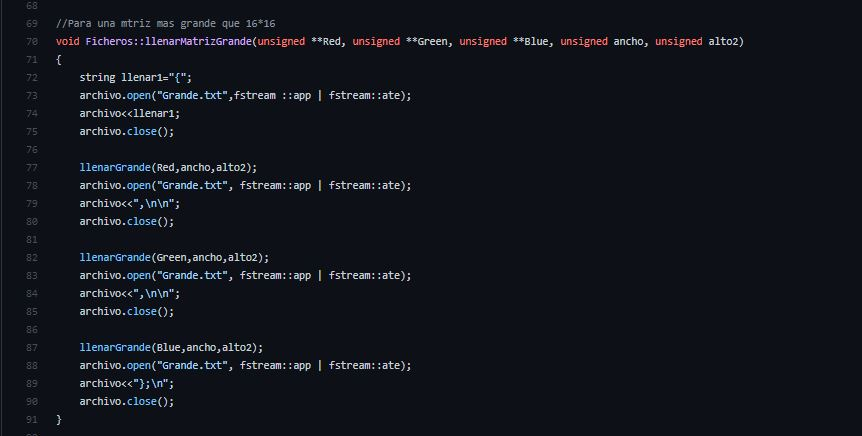
\includegraphics[width=10cm]{Imagenes/Metodos de la clase ficheros3.png}
\centering
\caption{Metodos de la clase ficheros}
\label{fig:Metodos de la clase fichero}
\end{figure}

\begin{figure}[ht]
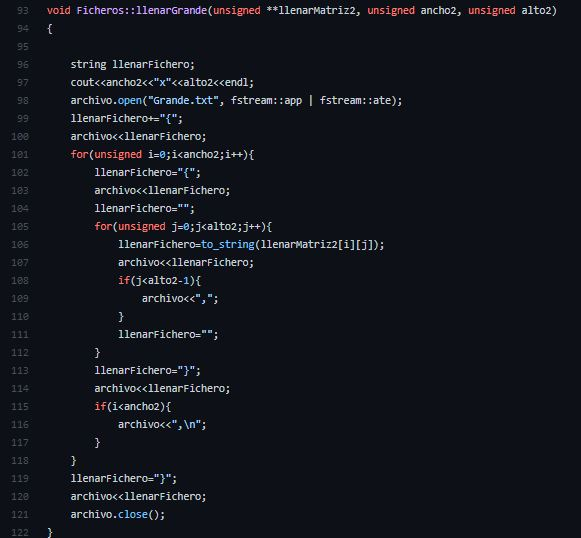
\includegraphics[width=10cm]{Imagenes/Metodos de la clase ficheros4.png}
\centering
\caption{Metodos de la clase ficheros}
\label{fig:Metodos de la clase fichero}
\end{figure}




\end{document}